	\subsection{UC 1 - Web App - Autenticazione}

%	\begin{figure}[H]
%		\centering
%		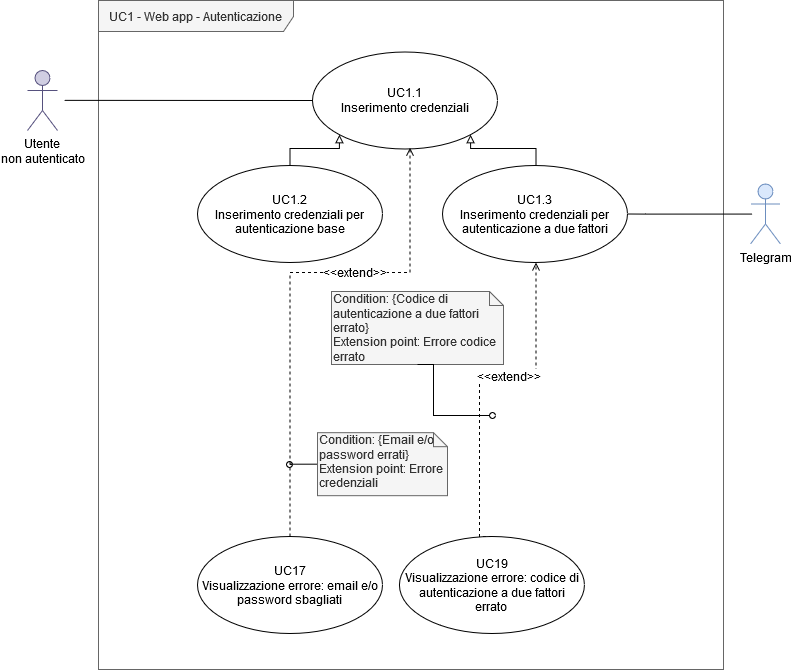
\includegraphics[scale=0.60]{res/images/uc1}
%		\caption{Diagramma che riassume il processo di autenticazione nella web app.}
%	\end{figure}

	\begin{itemize}
		\item \textbf{attori primari:} utente non autenticato;
%		\item \textbf{attori secondari:} \glock{Telegram};
		\item \textbf{descrizione:} l'utente vuole autenticarsi nella web app, per poter accedere alle funzionalità del sito e deve inserire alcuni campi obbligatori per procedere;
		\item \textbf{precondizione:} l'utente non è autenticato nella web app;
		\item \textbf{postcondizione:} l'utente effettua l'autenticazione nella web app;
		\item \textbf{scenario principale:}
		\begin{enumerate}
			\item l'utente inserisce le proprie credenziali, richieste per l'autenticazione nella web app;
		\end{enumerate}
		\item \textbf{estensioni:}
		\begin{itemize}
			\item visualizzazione errore: email e/o una password errati (UC 17);
			\item visualizzazione errore: account non autorizzato (UC 18);
		\end{itemize}
		\item \textbf{specializzazioni:}
		\begin{itemize}
			\item l'utente inserisce le credenziali per l'autenticazione base (UC 25);
			\item l'utente inserisce le credenziali per l'autenticazione a due fattori (UC 26).
		\end{itemize}
	\end{itemize}

